%======================
% Data Fitting
%======================

\documentclass{article}%
\usepackage{amsmath}
\usepackage{amsfonts}
\usepackage{amssymb}
\usepackage{graphicx}
\usepackage{fullpage}
\allowdisplaybreaks
\newtheorem{theorem}{Theorem}
\newtheorem{acknowledgement}[theorem]{Acknowledgement}
\newtheorem{algorithm}[theorem]{Algorithm}
\newtheorem{axiom}[theorem]{Axiom}
\newtheorem{case}[theorem]{Case}
\newtheorem{claim}[theorem]{Claim}
\newtheorem{conclusion}[theorem]{Conclusion}
\newtheorem{condition}[theorem]{Condition}
\newtheorem{conjecture}[theorem]{Conjecture}
\newtheorem{corollary}[theorem]{Corollary}
\newtheorem{criterion}[theorem]{Criterion}
\newtheorem{definition}[theorem]{Definition}
\newtheorem{example}[theorem]{Example}
\newtheorem{exercise}[theorem]{Exercise}
\newtheorem{lemma}[theorem]{Lemma}
\newtheorem{notation}[theorem]{Notation}
\newtheorem{problem}[theorem]{Problem}
\newtheorem{proposition}[theorem]{Proposition}
\newtheorem{remark}[theorem]{Remark}
\newtheorem{solution}[theorem]{Solution}
\newtheorem{summary}[theorem]{Summary}
\iffalse
\newenvironment{proof}{\noindent{\em Proof:}}{$\Box$~\\}
\fi
\setlength{\tabcolsep}{10pt}
\renewcommand{\arraystretch}{1.5}
\begin{document}

\title{Data Fitting}
\author{Grant McNaughton}
\date{10 February 2024}
\maketitle

We informally describe the data fitting problem by the following plots.

\begin{center}%
\begin{tabular}
[c]{ccc}
&
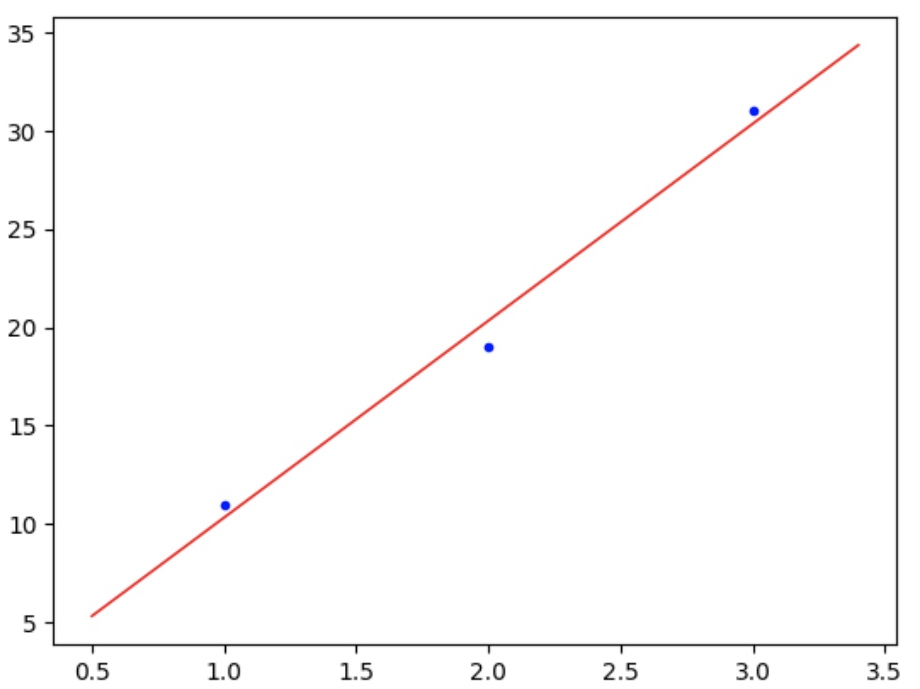
\includegraphics[
%trim=0.000000in 0.000000in 1.915576in -0.094059in,
%natheight=3.674200in,
%natwidth=5.674100in,
height=1.927in,
width=1.927in
]
{ex1.png}
&
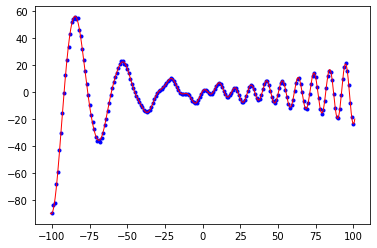
\includegraphics[
%trim=0.000000in 0.000000in 3.573603in 1.662208in,
%natheight=3.674200in,
%natwidth=5.585500in,
height=1.927in,
width=1.927in
]
{ex2.png}
\\
\\
&
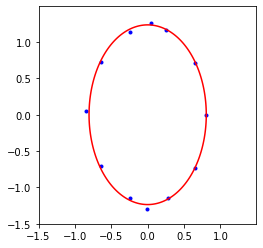
\includegraphics[
%trim=0.000000in 0.000000in 1.883958in 1.662208in,
%natheight=3.674200in,
%natwidth=3.896500in,
height=1.927in,
width=1.927in
]
{ex3.png}
&
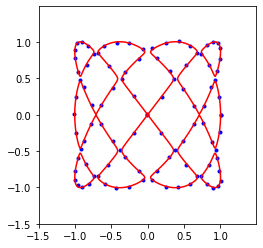
\includegraphics[
%trim=0.000000in 0.000000in 1.883958in 1.662208in,
%natheight=3.674200in,
%natwidth=3.896500in,
height=1.927in,
width=1.927in
]
{ex4.png}
\end{tabular}

\end{center}

\noindent Roughly put, the problem is, given \textquotedblleft
data\textquotedblright\ (blue points), find a \textquotedblleft
model\textquotedblright(red curve) that fits the data \textquotedblleft
well\textquotedblright. A few remarks.

\begin{enumerate}
\item The above plots are on the plane (2-dim space). However, many real-life
problems involve higher dimension space. Thus we will need to develop theory
and algorithms for arbitrary dimension.

\item Note that the top two cases could be fitted to a form $y=f\left(
x\right)  $ (\textquotedblleft functional\textquotedblright\ model) , while
the bottom two could not be fitted naturally to a functional model and hence
we will need to fit to a form $f\left(  x_{1},x_{2}\right)  =0$
(\textquotedblleft relational\textquotedblright\ model). Hence we will divide
the paper into two parts: functional model and relational model.

\item In order to solve the problems, we will need to make the informal
notions such as \textquotedblleft data\textquotedblright, \textquotedblleft
model\textquotedblright\ and \textquotedblleft well\textquotedblright. This is
what we will do in the following.
\end{enumerate}

\part{Functional Model}

%-----------------------------------------------------------


\section{Problem}

We will search for a good $f$ from linear combinations of a given model basis
functions $b=\left(  b_{1},\ldots,b_{n}\right)  $. Then we have the following
statement of the problem.

\begin{problem}
\ \ %

\begin{tabular}
[c]{lll}%
\text{In:} & $x\in\mathbb{R}^{m\times d},\ \ y\in\mathbb{R}^{m}$ & $m$ points
in $d\,$-dim space\ and corresponding values\\
& $b\in\mathbb{R}^{d}\rightarrow\mathbb{R}^{n}$ & model basis functions\\
\text{Out:} & $c\in\mathbb{R}^{n}\ \,$such that $f=bc$ fits $\left(
x,y\right)  $ well. & linear combination coefficients
\end{tabular}

\end{problem}

\begin{example}
[Running]\ We will use the following as a running example throughout this part.%
\\
\\
\begin{tabular}[c]{ll}%
\text{Input:} & $x=
\begin{bmatrix}
1\\
2\\
3
\end{bmatrix}  \in\mathbb{R}^{3\times1},\ y=
\begin{bmatrix}
11\\
19\\
31
\end{bmatrix} \in\mathbb{R}^{3}$, \ $b=
\begin{bmatrix}
x & 1
\end{bmatrix} \in\mathbb{R}^{1}\rightarrow\mathbb{R}^{2}$\\
\\
\bigskip
\text{Output:} & $c=
\begin{bmatrix}
10\\
\frac{1}{3}
\end{bmatrix}
\in\mathbb{R}^{2}$\\
& giving  $f=bc=10x+\frac{1}{3}$%
\end{tabular}

\begin{center}
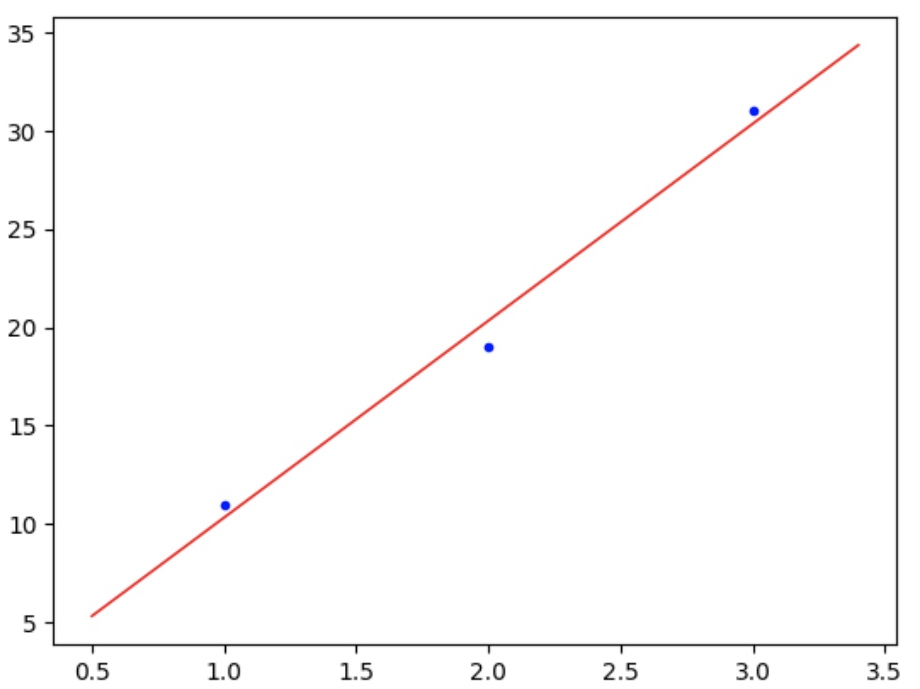
\includegraphics[scale = 0.2]{ex1.png}
\end{center}
\end{example}

\section{Theory}

\begin{notation}
\ We will use the following notations.

\begin{enumerate}
\item $x=\left[
\begin{array}
[c]{c}%
x_{1}\\
\vdots\\
x_{m}%
\end{array}
\right]  =\left[
\begin{array}
[c]{ccc}%
x_{11} & \cdots & x_{1d}\\
\vdots &  & \vdots\\
x_{m1} & \cdots & x_{md}%
\end{array}
\right]  $

\item $y=\left[
\begin{array}
[c]{c}%
y_{1}\\
\vdots\\
y_{m}%
\end{array}
\right]  $

\item $b=\left[
\begin{array}
[c]{ccc}%
b_{1} & \cdots & b_{n}%
\end{array}
\right]  $

\item $c=\left[
\begin{array}
[c]{c}%
c_{1}\\
\vdots\\
c_{m}%
\end{array}
\right]  $
\end{enumerate}
\end{notation}

\subsection{Reducing data fitting to over-determined system solving}

We need to find $c$ such that%
\begin{align*}
y_{1} &  =c_{1}b_{1}\left(  x_{1}\right)  +\cdots+c_{n}b_{n}\left(
x_{1}\right)  \\
&  \vdots\\
y_{m} &  =c_{1}b_{1}\left(  x_{m}\right)  +\cdots+c_{n}b_{n}\left(
x_{m}\right)
\end{align*}
Using matrix/vector, we have%
\[
\begin{bmatrix}
y_1\\
\vdots\\
y_m
\end{bmatrix}
=
\begin{bmatrix}
b_1\left(  x_{1}\right)   & \cdots & b_n\left(  x_1\right)  \\
\vdots &  & \vdots\\
b_1\left(  x_m\right)   & \cdots & b_n\left(  x_m\right)
\end{bmatrix} 
\begin{bmatrix}
c_1\\
\vdots\\
c_n%
\end{bmatrix}
\]
Compactly put, we have%
\[
y=Bc
\]
where%
\[
B=
\begin{bmatrix}
b_1\left(  x_{1}\right)   & \cdots & b_n\left(  x_1\right)  \\
\vdots &  & \vdots\\
b_1\left(  x_m\right)   & \cdots & b_n\left(  x_m\right)
\end{bmatrix} 
\in\mathbb{R}^{m\times n}
\]
is the ``generalized Vandermonde matrix''.
Thus we have reduced the data fitting problem to the linear system of
equations solving.%

\begin{tabular}[c]{ll}
\text{Input:} & $B\in\mathbb{R}^{m\times n}$\\
& $y\in\mathbb{R}^{m}$\\
Output: & $c\in\mathbb{R}^{n}\ \ $such that $y=Bc$%
\end{tabular}


\noindent Note that usually $m\gg n$. Hence we have over-constrained problem.
Hence  in general there is no solution. Hence, we will try to find $c$ which
is \textquotedblleft close\textquotedblright\ to being a solution. The
following subsection elaborate on this.

\subsection{Solving over-constrained system}
% hint: establish the projection of y onto the column space of B which can be used to choose the best c

From our equation $Bc=y$ we want to find $\Bar{c}=My$ for some matrix computation $M$. To do this, we can use the following logic:

\begin{align*}
    B\Bar{c} &= y\\
    B^\intercal B\Bar{c} &= B^\intercal y\\
    (B^\intercal B)^{-1} (B^\intercal B) \Bar{c} &= (B^\intercal B)^{-1} B^\intercal y\\
    \Bar{c} &= (B^\intercal B)^{-1} B^\intercal y
\end{align*}

Note that we must use $B^\intercal B$ instead of just $B$ to ensure the matrix is invertible. This allows us to find an approximation of $c$ even though our system is overconstrained and has no perfect solution.

\subsection{Solving over-constrained system via SVD}

% hint: follow lecture notes on SVD, and fill in the intermediate steps

As $B$ grows, it quickly becomes computationally costly to find $(B^\intercal B)^{-1}$. One way to avoid this problem is to use singular value decomposition, which is much easier for large matrices $B$.

Let us first define $B$ with the singular value decomposition $B=U\Sigma V^\intercal$ for an orthogonal matrix $U$ composed of the left singular vectors of $BB^\intercal$, an orthogonal matrix $V$ composed of the right singular vectors of $B^\intercal B$, and a diagonal matrix $\Sigma$ composed of the singular values of $B$.
The singular vectors and values are defined as the set of eigenvectors and eigenvalues satisfying $BB^\intercal u_i = \sigma^2_i u_i$ or $B^\intercal B v_i = \sigma^2_i v_i$.

We can also describe $B$ as
\[
B = U \Sigma V^\intercal = \begin{bmatrix}
    \vline & \vline & & \vline \\
    \vline & \vline & & \vline \\
    u_1 & u_2 & \dots & u_m\\
     \vline & \vline & & \vline \\
     \vline & \vline & & \vline \\
\end{bmatrix} \begin{bmatrix}
    \sigma_1 & 0 & \hdots & 0 & 0 & \hdots & 0\\
    0 & \sigma_2 & \hdots & 0 & 0 & \hdots & 0\\
    \vdots & \vdots & \ddots & \vdots & \vdots& & \vdots \\
    0 & 0 & \hdots & \sigma_r & 0 & \hdots & 0\\
    0 & 0 & \hdots & 0 & 0 & \hdots & 0\\
    \vdots & \vdots & & \vdots & \vdots &\ddots & \vdots\\
    0 & 0 & \hdots & 0 & 0 & \hdots & 0
\end{bmatrix} \begin{bmatrix}
    \textbf{------} & v_1^\intercal & \textbf{------}\\
        \textbf{------} & v_2^\intercal & \textbf{------}
\\     & \vdots & 
\\   \textbf{------} & v_n^\intercal & \textbf{------}

\end{bmatrix}
\]
We can then perform the following calculations to get our SVD-based model fitting:
\begin{align*}
    \Bar{c} &= (B^\intercal B)^{-1} B^\intercal y \\
    &= ((U \Sigma V^\intercal)^\intercal (U \Sigma V^\intercal))^{-1} V \Sigma U^\intercal y\\
    &= (V \Sigma U^\intercal U \Sigma V^\intercal)^{-1} V \Sigma U^\intercal y\\
    &= (V^\intercal)^{-1} \Sigma^{-1} U^{-1} (U^\intercal)^{-1} \Sigma^{-1} V^{-1} V \Sigma U^\intercal y\\
    &= (V^\intercal)^{-1} \Sigma^{-1} U^{-1} y\\
    &= V \Sigma^{-1} U^\intercal y
\end{align*}
Note that because $U$ and $V$ are orthogonal, $U^\intercal=U^{-1}$ and $V^\intercal=V^{-1}$. This final $\Bar{c}$ can be used to quickly calculate our model.
\section{Algorithm}

\begin{algorithm}
\ 

\begin{enumerate}
\item $x = \begin{bmatrix}
    \textbf{---} & x_1 & \textbf{---}\\
     & \vdots & \\
     \textbf{---} & x_m & \textbf{---}
\end{bmatrix}, y=\begin{bmatrix}
    y_1 \\ \vdots \\ y_m
\end{bmatrix}, b = \begin{bmatrix}
    b_1(x) & \cdots & b_n(x)
\end{bmatrix}$
\item $B=
\begin{bmatrix}
b_1\left(  x_{1}\right)   & \cdots & b_n\left(  x_1\right)  \\
\vdots &  & \vdots\\
b_1\left(  x_m\right)   & \cdots & b_n\left(  x_m\right)
\end{bmatrix}$

\item $U, \Sigma, V = \textnormal{SVD} (B)$

\item $\Bar{c} = V \Sigma^{-1} U^\intercal y$
\end{enumerate}
\end{algorithm}

\begin{example}
\ 

\begin{enumerate}
\item $x\leftarrow
\begin{bmatrix}
1\\
2\\
3
\end{bmatrix}, y\leftarrow \begin{bmatrix}
   11\\19\\31 
\end{bmatrix}, b \leftarrow \begin{bmatrix}
    x & 1
\end{bmatrix}$

\item $B \leftarrow \begin{bmatrix}
    1 & 1\\
    2 & 1\\
    3 & 1
\end{bmatrix}$

\item $U, \Sigma, V \leftarrow \text{SVD}(B) \approx \begin{bmatrix}
    -.85 & .32 & .41 \\
    -.18 & .55 & -.82 \\
    .49 & .77 & .41
\end{bmatrix}, \begin{bmatrix}
    .6 & 0 \\
    0 & 4.08 \\
    0 & 0
\end{bmatrix}, \begin{bmatrix}
    -.91 & .4 \\
    .4 & .91
\end{bmatrix}$
\item $\Bar{c} \leftarrow \begin{bmatrix}
    \frac{1}{3} \\ 10
\end{bmatrix}$
\end{enumerate}
\end{example}
\pagebreak
\part{Relational Model}

% Now you are on your own. Fill in this section in a similar style! You don't need to do an example for this section.

\section{Problem}

We will search for a good $b$ from linear combinations of a given model basis
functions $b=\left(  b_{1},\ldots,b_{n}\right)  $. Then we have the following
statement of the problem.

\begin{problem}
\ \ %

\begin{tabular}
[c]{lll}%
\text{In:} & $x\in\mathbb{R}^{m\times d}$ & $m$ unlabeled points in $d\,$-dim space\\
& $b\in\mathbb{R}^{d}\rightarrow\mathbb{R}^{n}$ & model basis functions\\
\text{Out:} & $c\in\mathbb{R}^{n}\ \,$such that $f=bc$ fits $\left(
x,y\right)  $ well. & linear combination coefficients
\end{tabular}

\end{problem}

\section{Theory}

\subsection{Idea of unlabeled relation fitting}

We need to find $c$ such that $c_1 b_1 (x) + c_2 b_2 (x) + \dots + c_n b_n (x) = 0$. Using matrix/vector notation, we have
\[
\begin{bmatrix}
    b_1(x_1) & \cdots & b_n(x_1) \\
    \vdots & \ddots & \vdots \\
    b_1(x_m) & \cdots & b_n(x_n)
\end{bmatrix} \begin{bmatrix}
    c_1 \\ \vdots \\ c_n
\end{bmatrix} = 0
\]

Compactly put, we have%
\[
Bc=0
\]
where, once again,%
\[
B=
\begin{bmatrix}
b_1\left(  x_{1}\right)   & \cdots & b_n\left(  x_1\right)  \\
\vdots &  & \vdots\\
b_1\left(  x_m\right)   & \cdots & b_n\left(  x_m\right)
\end{bmatrix} 
\in\mathbb{R}^{m\times n}
\]
is the ``generalized Vandermonde matrix''.

\subsection{Issues with this method}
This method of relation fitting presents two main issues. The first of these issues is that the trivial solution ${c}=\vec{0}$ will always fit our model as the easiest to compute result. To deal this this challenge, we will set $||{c}||= 1$, preventing $\vec{0}$ from being a possible solution.

The second main issue with our proposed method of relation fitting is that, once again, usually $m \gg n$. As with function fitting, we can best solve our overconstrained system by minimizing $||B{c}||$ for our system instead of finding $B, c$ such that $||Bc||=\vec{0}$.

\subsection{Solving the relation fitting problem via eigendecomposition}

Consider $||Bc||=(Bc)^\intercal Bc$. Let $S=B^\intercal B$ and $||Bc||=c^\intercal B^\intercal B c = c^\intercal S c$. Set $V, \Lambda = \textnormal{eigendecomposition}(S)$.

Because $S$ must be symmetric based on its definition, all of its eigenvalues $\lambda_1, \dots , \lambda_n$ are real and all eigenvector columns of $V$ are orthogonal. Because $V$ is an orthonormal matrix, we can express $c$ as a linear combination of its vectors as follows:
\[
c=a_1 v_1 + a_2 v_2 + \dots + a_n v_n
\]
for some $a_1, a_2, \dots, a_n$. Let us now return to our main problem,
\begin{align*}
    \textnormal{min} (c^\intercal S c )&=c^\intercal S (a_1 v_1 + a_2 v_2 + \dots + a_n v_n)\\
    &=c^\intercal (Sa_1 v_1 + Sa_2 v_2 + \dots + Sa_n v_n)\\
    &=c^\intercal (a_1 S v_1 + a_2 S v_2 + \dots + a_n S v_n)\\
    &=c^\intercal (a_1 \lambda_1 v_1 + a_2 \lambda_2 v_2 + \dots + a_n \lambda_n v_n)\\
    &= (a_1 v_1^\intercal + a_2 v_2^\intercal + \dots + a_n v_n^\intercal)(a_1 \lambda_1 v_1 + a_2 \lambda_2 v_2 + \dots + a_n \lambda_n v_n)
\end{align*}
Because all vectors $v_i$ are orthogonal, $v_i ^\intercal v_i =1$ and $v_i^\intercal v_j = 0$ for all $i,j$ in $[1,n]$. Thus we can continue our computation
\begin{align*}
    \textnormal{min} (c^\intercal S c )&=(a_1 v_1^\intercal + a_2 v_2^\intercal + \dots + a_n v_n^\intercal)(a_1 \lambda_1 v_1 + a_2 \lambda_2 v_2 + \dots + a_n \lambda_n v_n)\\
    &= \lambda_1 a_1^2 + \lambda_2 a_2^2 + \dots + \lambda_n a_n^2
\end{align*}
Without loss of generality, let the eigenvalues $\lambda_i$ be sorted such that $\lambda_1 \geq \lambda_2 \geq \dots \geq \lambda_n$. We also know that $||c||=1$, thus $\sum_{i=1}^n a_i^2 =1$. We can use this to reach the final conclusion that
\begin{align*}
\textnormal{min}(||Bc||)&=\textnormal{min}(c^\intercal S c) \\&= \textnormal{min}(\lambda_1 a_1^2 + \lambda_2 a_2^2 + \dots + \lambda_n a_n^2)\\ &= 0 \cdot \lambda_1 + 0 \cdot \lambda_2 + \dots + 0 \cdot lambda_{n-1} + 1 \cdot \lambda_n\\
&= \lambda_n
\end{align*}
Thus $c^\intercal S c$ is minimized exactly when $c$ is the eigenvector corresponding to the smallest eigenvalue of $S$.

\section{Algorithm}
\begin{enumerate}
    \item $x = \begin{bmatrix}
    \textbf{---} & x_1 & \textbf{---}\\
     & \vdots & \\
     \textbf{---} & x_m & \textbf{---}
\end{bmatrix}, b = \begin{bmatrix}
    b_1(x) & \cdots & b_n(x)
\end{bmatrix}$

\item $B=
\begin{bmatrix}
b_1\left(  x_{1}\right)   & \cdots & b_n\left(  x_1\right)  \\
\vdots &  & \vdots\\
b_1\left(  x_m\right)   & \cdots & b_n\left(  x_m\right)
\end{bmatrix}$

\item $S=B^\intercal B$
\item $\Lambda, V = \textnormal{eigendecomposition}(S)$
\item $k=$ index of the smallest eigenvalue of $S$
\item $c = k^\textnormal{th}$ eigenvector

\end{enumerate}
\end{document}
